\documentclass{article}

% Language setting
% Replace `english' with e.g. `spanish' to change the document language
\usepackage[french]{babel}
\usepackage[fleqn]{amsmath} % Aligner les équations à gauche


% Set page size and margins
% Replace `letterpaper' with`a4paper' for UK/EU standard size
\usepackage[letterpaper,top=2cm,bottom=2cm,left=3cm,right=3cm,marginparwidth=1.75cm]{geometry}

% Useful packages

\usepackage{amsmath}
\usepackage{graphicx}
\usepackage{subcaption}
\usepackage[colorlinks=true, allcolors=blue]{hyperref}

\title{TD Michelson }
\author{IPESUP - PC }
\date{DATE}

\begin{document}
\maketitle

\section{Rappels de cours}

Il existe deux réglages du Michelson, en \textbf{lame d'air} et en \textbf{coin d'air}. 
En lame d'air: \\
\begin{itemize}
  \item Les miroirs sont perpendiculaires
  \item Les franges sont localisées à l'infini (penser à regarder "au loin" pour les observer à l'oeil nu)
  \item $\delta = 2ne cos(i)$ 
  \item La figure d'interférences est faite d'anneaux (franges d'égale inclinaison). \\

\end{itemize}

En coin d'air: \\
\begin{itemize}
  \item Les miroirs ne sont pas perpendiculaires (angle $\alpha$). 
  \item Les franges sont situées au voisinage des miroirs. 
  \item $\delta = 2 \alpha x $
  \item Les franges sont des droites parallèles d'égale épaisseur. \\
\end{itemize}

Pour arriver au contact optique ($e=0$), on se place en configuration lame d'air et on rapproche les miroirs de façon à ce que les anneaux convergent vers le centre jusqu'à l'obtention de la teinte plate. 


\begin{figure}[htbp]
  \centering{
  \begin{subfigure}[b]{0.45\textwidth}
      \centering
      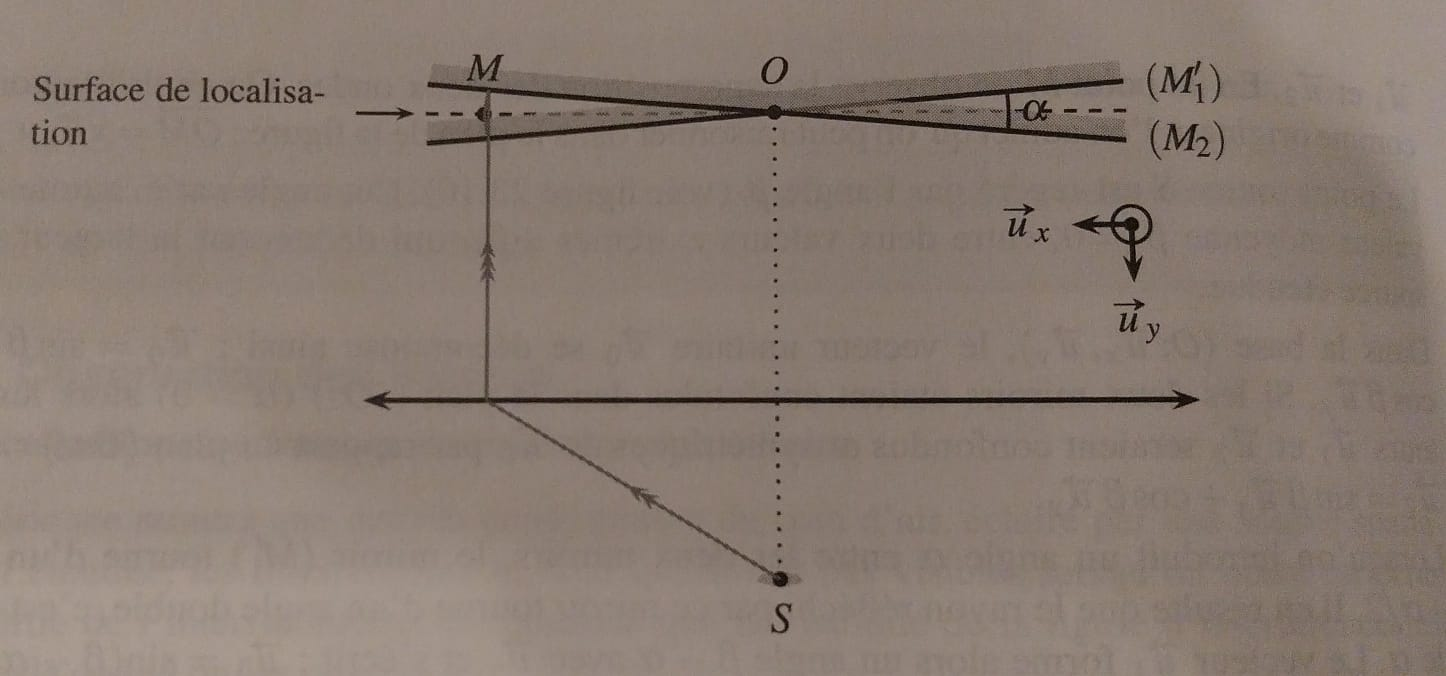
\includegraphics[width=\textwidth]{schema_michelson_coin_d_air.jpg}
      \caption{Michelson réglé en coin d'air}                                              
  \end{subfigure}
  \begin{subfigure}[b]{0.3\textwidth}
      \centering
      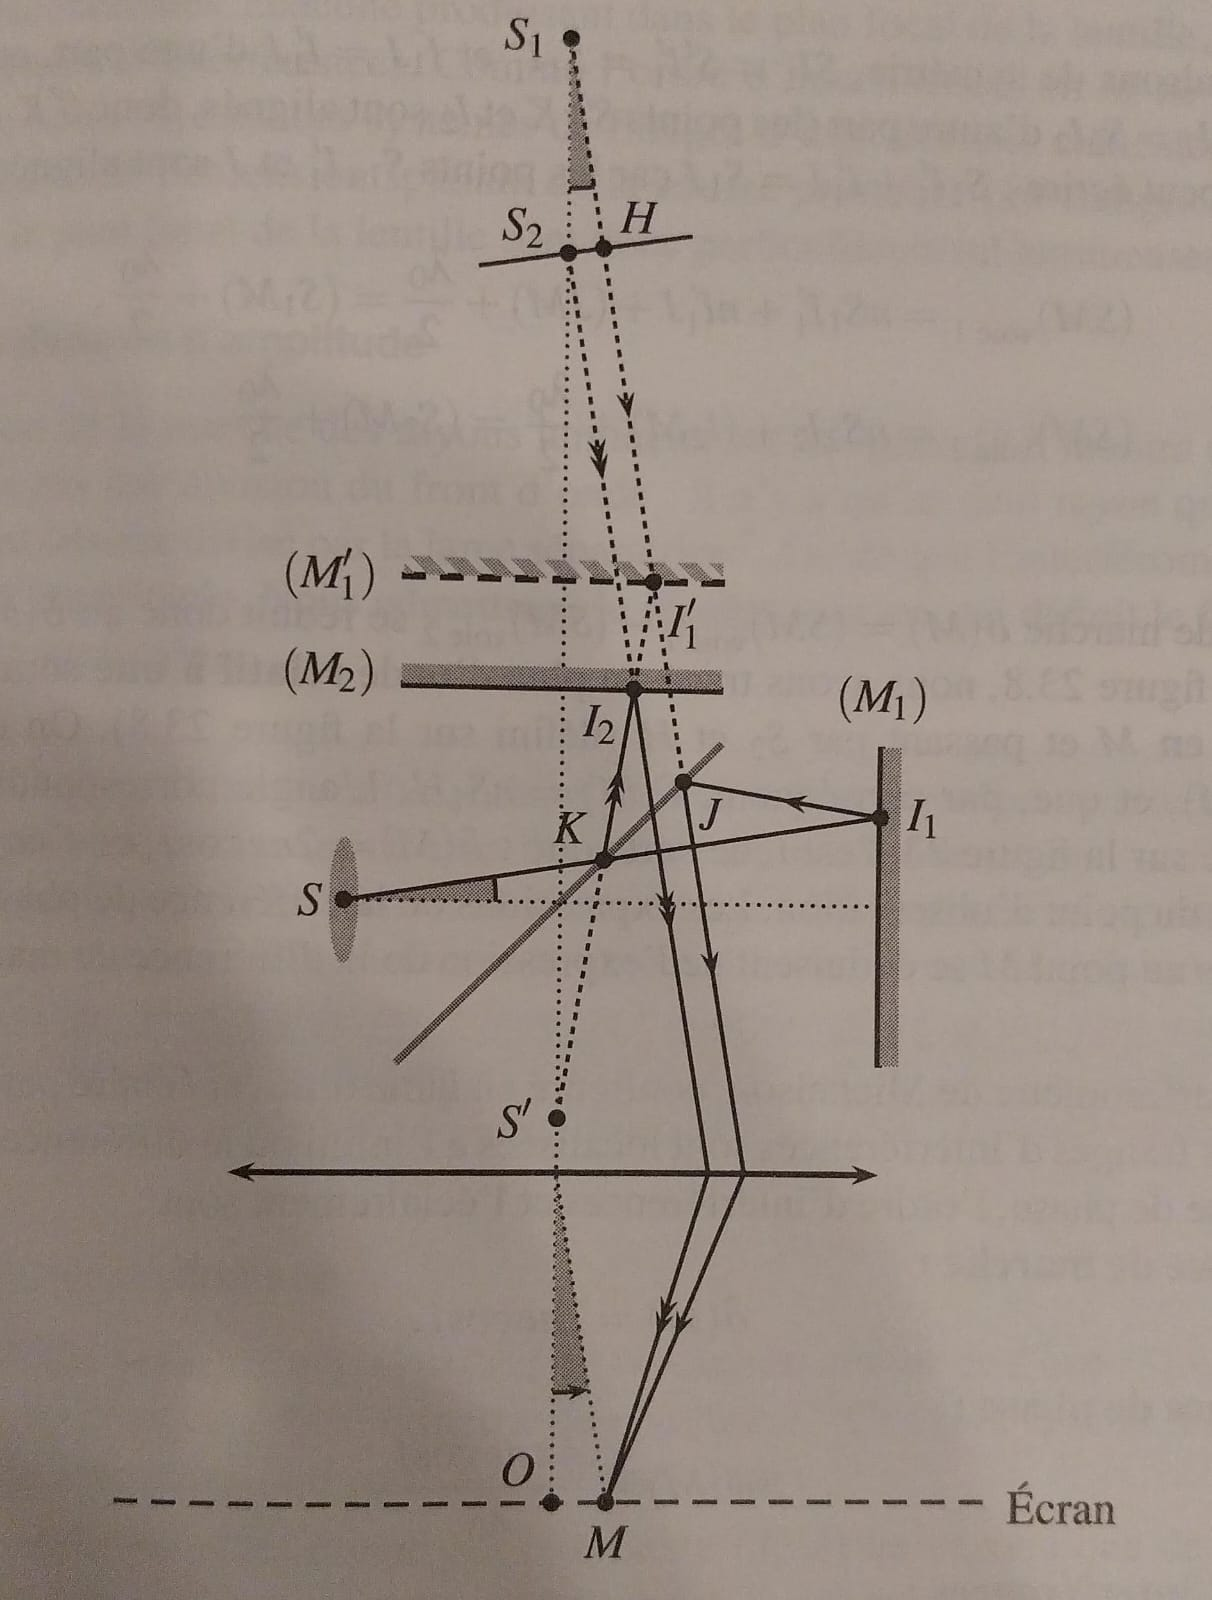
\includegraphics[width=\textwidth]{schema_michelson_lame_d_air.jpg}
      \caption{Michelson réglé en lame d'air } 
  \end{subfigure}}
  \caption{Deux manières de régler un Michelson}
\end{figure}




\begin{figure}[h!]
  \centering{
  \begin{subfigure}[b]{0.35\textwidth}
      \centering
      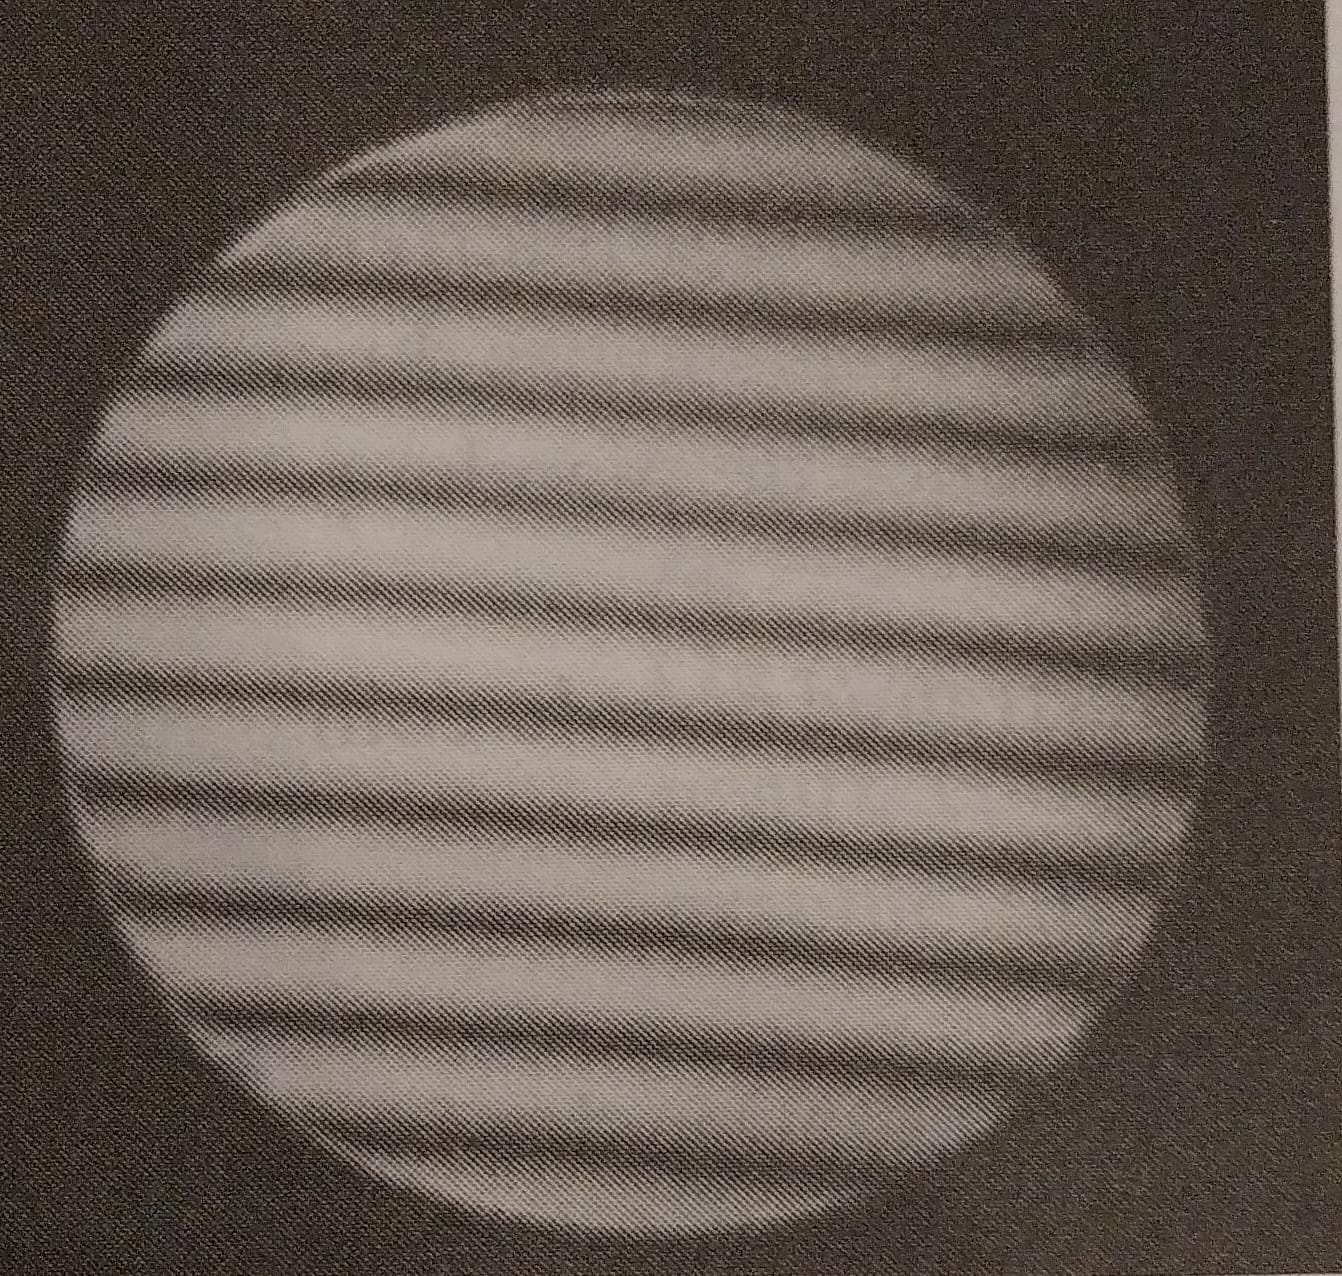
\includegraphics[width=\textwidth]{franges_egale_epaisseur.jpg}
      \caption{Franges d'égale épaisseur}                                              
  \end{subfigure}
  \begin{subfigure}[b]{0.3\textwidth}
      \centering
      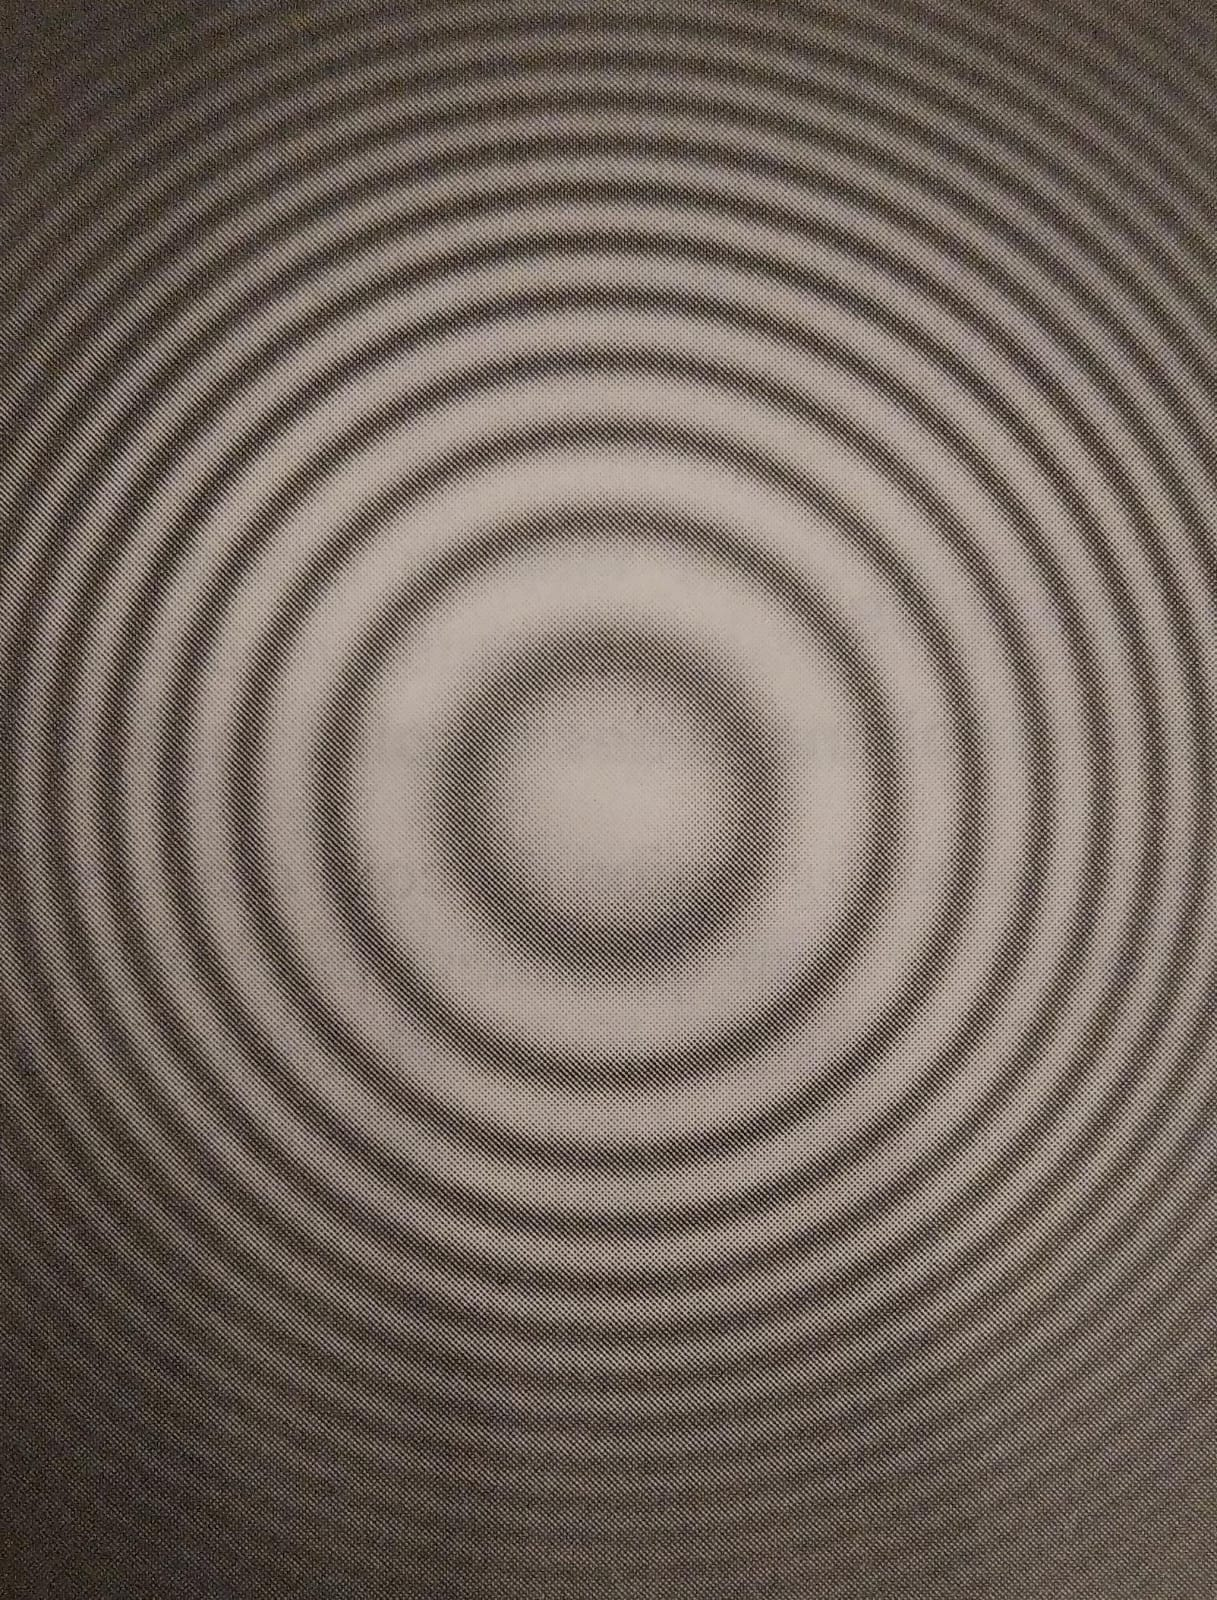
\includegraphics[width=\textwidth]{franges_anneaux.jpg}
      \caption{Franges d'égale inclinaison }
      \label{fig:franges_egales_epaisseur}
  \end{subfigure}}
  \caption{Les observations associées aux différents réglages}
\end{figure}


\newpage
\section{Anneaux d'égale inclinaison}

Un interféromètre de Michelson est réglé en lame d'air et éclairé avec une lampe à vapeur de sodium, qu'on considérera monochromatique, de longueur d'onde $\lambda = 589nm$.
On observe sur un écran un ensemble d'anneaux concentriques (voir Fig \ref{fig:franges_egales_epaisseur}). 
\begin{enumerate}
  \item Préciser l'ensemble des réglages nécessaires à l'obtention des anneaux visibles sur la figure \ref{fig:franges_egales_epaisseur}. 
  \item Un logiciel permet de tracer le profil des niveaux de gros de la figure \ref{fig:franges_egales_epaisseur} selon un diamètre vertical. Le résultat est donné Fig. \ref{fig:niveaux_de_gris}. Déterminer la valeur $e$ de l'épaisseur entre les deux miroirs, sachant que les anneaux sont observé dans le plan focal d'une lentille convergente de distance focale $f'=1,00m$ placée en sortie de l'interféromètre.
  \item Si on réduit $e$ de moitié, combien d'anneaux vont défiler au centre de la figure d'interférences ?  
\end{enumerate}

\begin{figure}
  \centering
  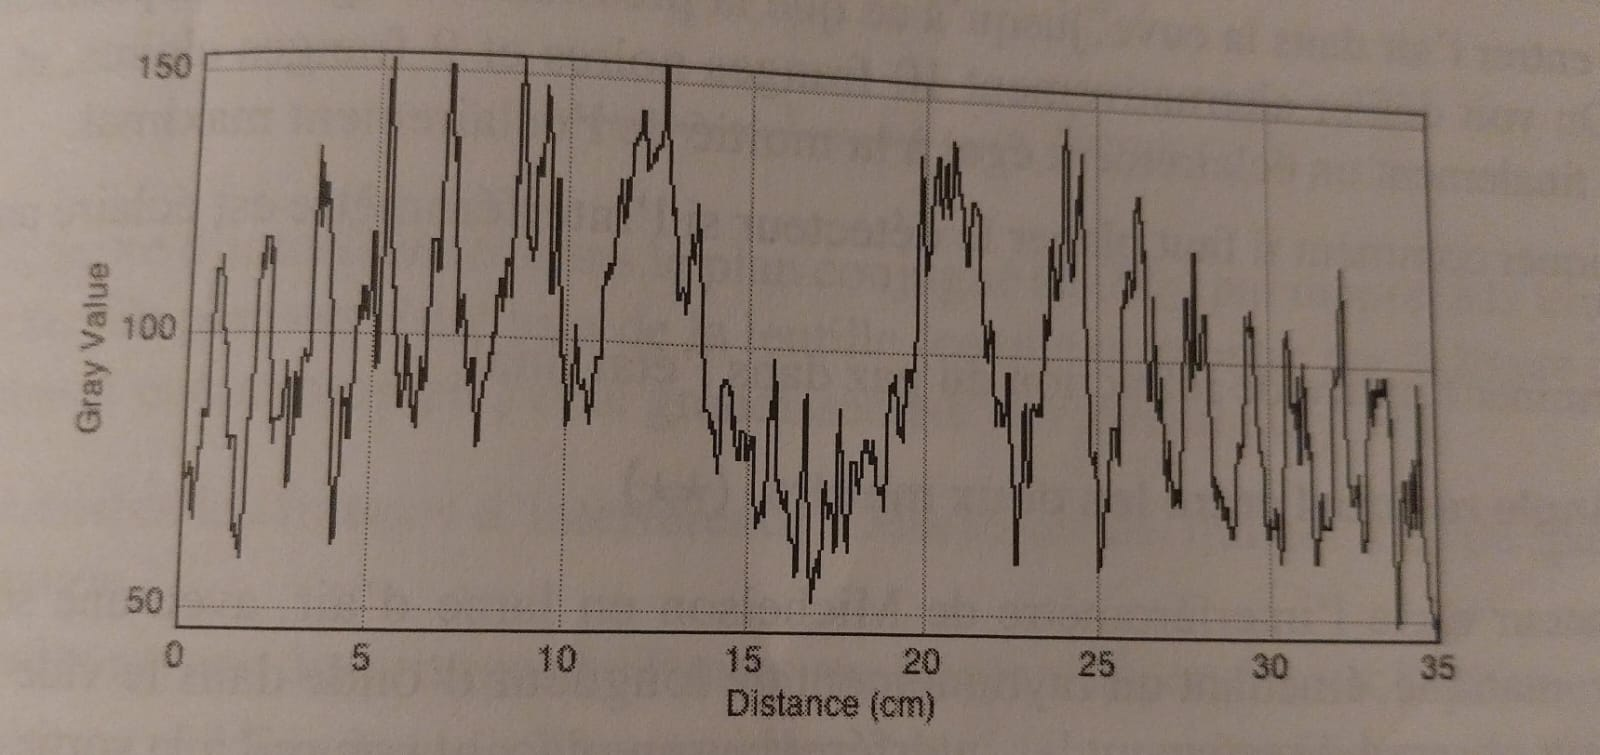
\includegraphics[width=0.5\textwidth]{niveaux_de_gris.jpg}
  \caption{Profil d'éclairement (l'axe des abscisses est en cm)}   
  \label{fig:niveaux_de_gris}
\end{figure}


\section{Mesure de l'écart du doublet jaune du sodium}

\end{document}

